\section{Processing Graphics}

\subsection{Getting Started}
\begin{frame}[fragile]{Installing}{}
\end{frame}

\begin{frame}[fragile]{}{}
    \Large
    \begin{minted}{c++}
        fill(0); //Set fill color
        ellipse(a, b, c, d);
    \end{minted}
    \pause
    \begin{minted}{text}
        a  float: x-coordinate of ellipse
        b  float: y-coordinate of ellipse
        c  float: width of the ellipse
        d  float: height of the ellipse
    \end{minted}
\end{frame}

\begin{frame}[fragile]{Window Size}{}
    \Large
    \begin{minted}{c++}
    int displayWidth = 800;
    int displayHeight = 400;
    \end{minted}
    \pause
    \begin{minted}{c++}
    size(displayWidth, displayHeight);
    \end{minted}
    \pause
    \begin{minted}{c++}
    // The wrong way to specify
    // the middle of the screen
    ellipse(400, 200, 50, 50);
    \end{minted}
    \pause
    \begin{minted}{c++}
    // Always the middle
    // no matter how size() changes
    ellipse(width/2, height/2, 50, 50);
    \end{minted}
\end{frame}

\subsection{Logic Flow}
\begin{frame}[fragile]{Flow}{}
\begin{figure}
    \begin{center}
        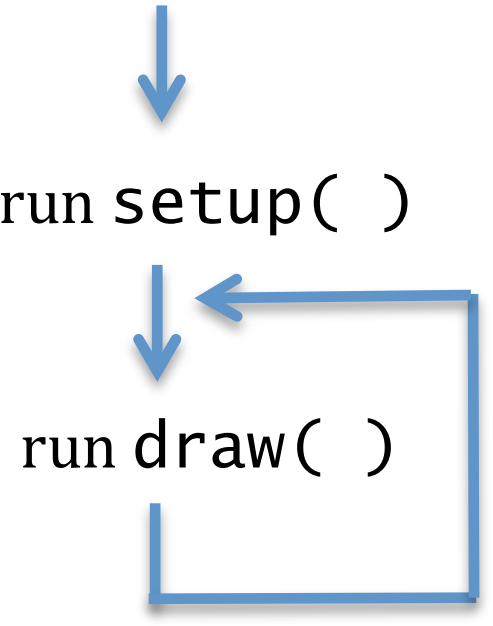
\includegraphics[width=0.8\linewidth]{images/setup_draw.png}
    \end{center}
\end{figure}
\end{frame}

\begin{frame}[fragile]{Setup and Loop}{}
    \begin{minted}{c++}
int displayWidth = 800;
int displayHeight = 400;
    \end{minted}
    \pause
    \begin{minted}{c++}
void setup (){
    size(displayWidth, displayHeight);
}
    \end{minted}
    \pause
    \begin{minted}{c++}
void draw (){
    background(255);
    fill(0);
    ellipse(width/2, height/2, 50, 50);
}
    \end{minted}
\end{frame}

